\documentclass[aspectratio=169]{beamer}
\beamertemplatenavigationsymbolsempty
\usepackage{qrcode}

\usepackage{parskip, setspace}
\setstretch{1.5}

\usepackage{biblatex}
\addbibresource{bib.bib}
% math formatting
\usepackage{amsmath, amsfonts, braket}
% \numberwithin{equation}{section}
% rich text
\usepackage{multimedia}
\usepackage{graphicx, caption}
\usepackage{hyperref}
\usepackage{xcolor}
\hypersetup{
    colorlinks=false,
    linkcolor=black,  
    urlcolor=blue,
    citecolor=blue,
    pdftitle={Chapman APS NW 2024},
    pdfpagemode=FullScreen,
}

\usepackage[ruled,linesnumbered,lined,boxed,commentsnumbered]{algorithm2e}

\usetheme{Madrid}
\title[Analog Particles with HPC]{Modelling Particle Production in Analog (3+1) Inflationary Cosmologies Using High-Performance Computing}
% \subtitle{}

\author[Chapman, Nathaniel]{Nathaniel Chapman}

\institute[CWU]
{
  Department of Computer Science \\
  Department of Physics \\
  Central Washington University
%   \and
%   \inst{2}%
%   Faculty of Chemistry\\
%   Very Famous University
}

\date[APS NW 2024]{APS NW 2024}

\logo{
\includegraphics[height=0.5cm]{images/cwu_logo.png}}

\begin{document}

\frame{\titlepage}
% \begin{frame}
%     \frametitle{Table of Contents}

%     \tableofcontents

% \end{frame}

\section{Introduction}
\subsection{}
\begin{frame}
    \frametitle{Introduction - Analog Universes}

    \begin{columns}
        \begin{column}{0.5\textwidth}
            \begin{enumerate}
                \item <1->Inflation created particles
                \item <2->Cannot directly observe these particles
                \item <3->Theory suggests phase fluctuations of ultra-cold quantum gases behave similarily
                \item <4->Can make gas in the lab $\implies$ can \emph{effectively} observe inflation particles
                \item <5->Lab based system = ``analog universe''
            \end{enumerate}
        \end{column}
        \begin{column}{0.5\textwidth}
            \begin{figure}
                \centering
                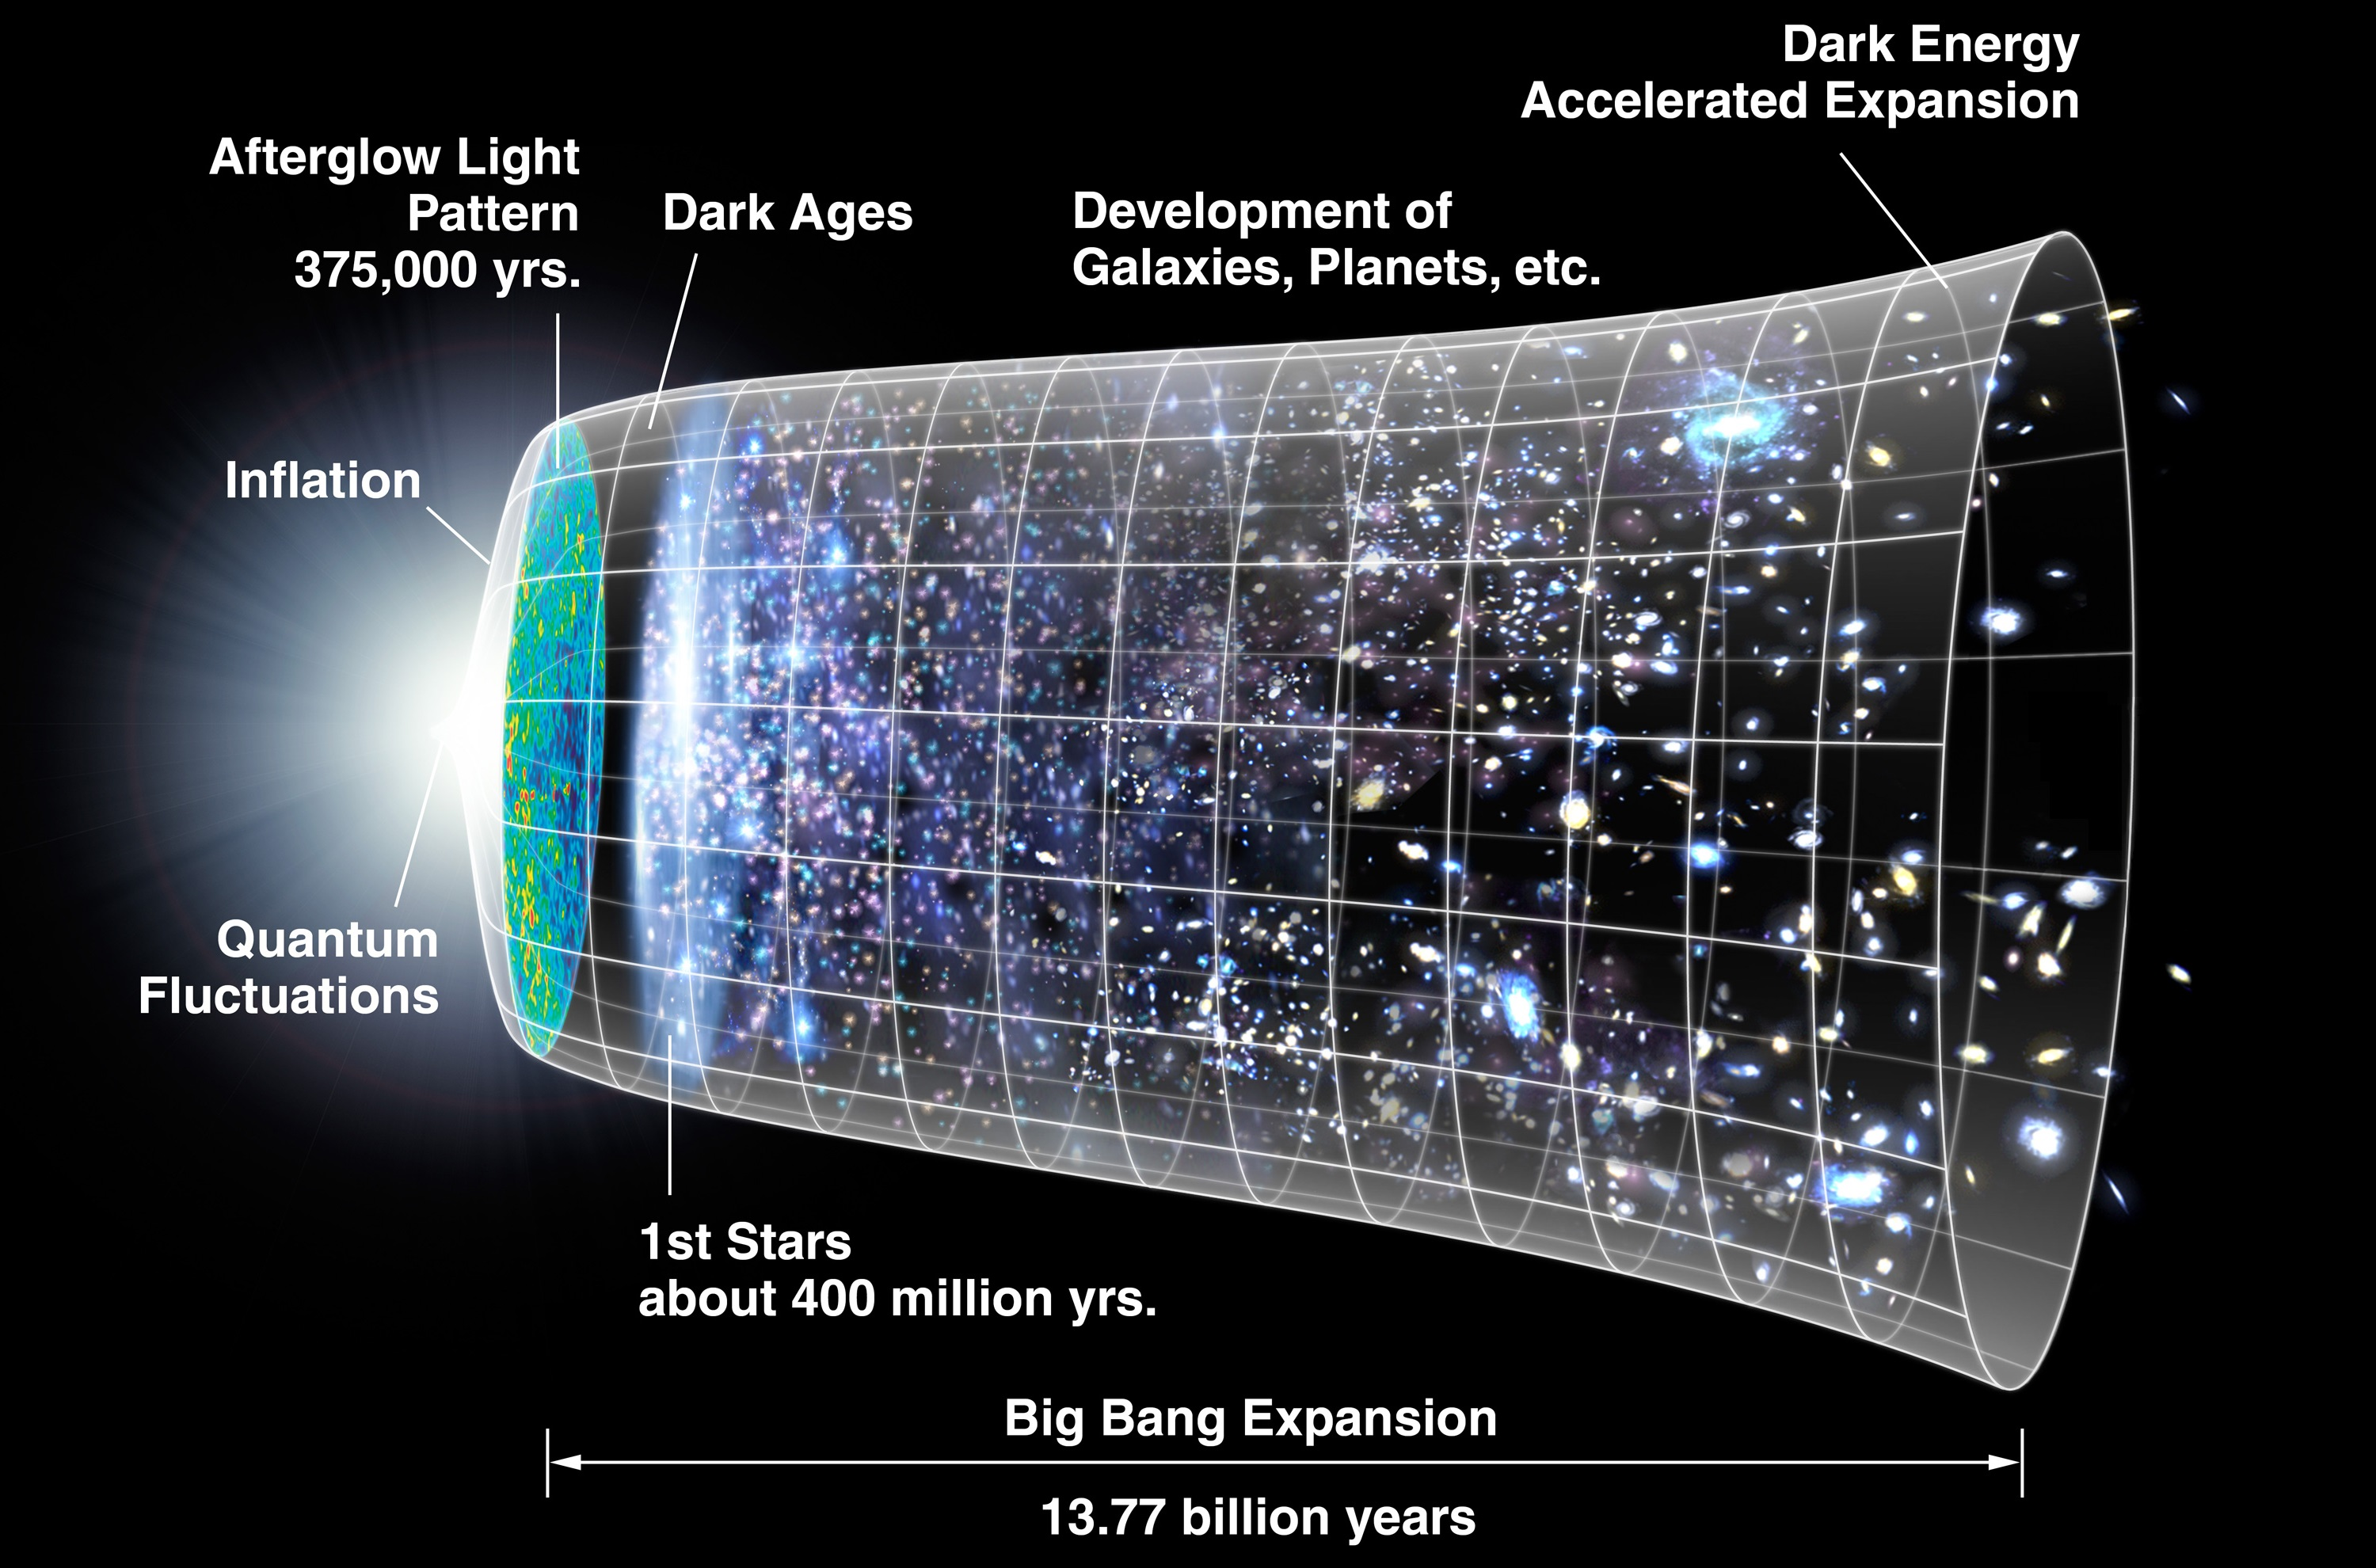
\includegraphics[width=\textwidth]{images/CMB_Timeline300_no_WMAP.jpg}
                \caption{History of the universe highlighting period of rapid expansion}
            \end{figure}
        \end{column}
    \end{columns}
    \footnotesize Source: \url{https://upload.wikimedia.org/wikipedia/commons/6/6f/CMB_Timeline300_no_WMAP.jpg}
\end{frame}

\begin{frame}
    \frametitle{Introduction - The Story So Far}

    \begin{columns}
        \begin{column}{0.5\textwidth}
            \begin{itemize}
                \item <1->Many investigations into analog universes e.g. Visser and Wienfurtner
                \item <2->Few investigations into exact analogs
                \item <3->Fewer into computational simulation
                \item <4->Even fewer using high-performance computing
            \end{itemize}
        \end{column}
        \begin{column}{0.5\textwidth}
            \begin{figure}
                \centering
                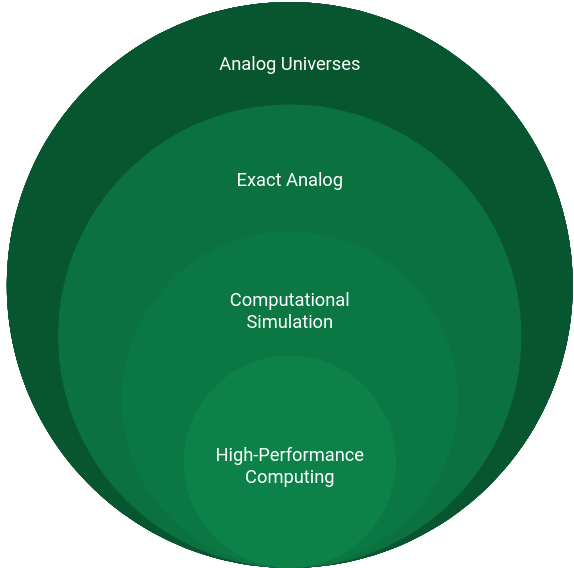
\includegraphics[width=0.7\textwidth]{images/subsets.png}
                \caption{Subsets of increasingly specific literature}
            \end{figure}
        \end{column}
    \end{columns}

\end{frame}

\section{Methods}

% \begin{frame}
%     \frametitle{Methods - Physical}

%     % \begin{itemize}
%     %     \item Excited quantum fields in curved spacetime: \\ massless, spin-0 quasiparticles arising from a non-unique Fock vacuum
%     %     \item Phase perturbations in ultra-cold quantum gas: \\ ground state Bose-Einstein condensate without thermal or quanutm fluctuations
%     %     \item Wave to particle transition: Trans-phononic cutoff (free-particle can be modeled by including quantum fluctuations)
%     %     \item Analog expansion comes from speed-space degeneracy
%     % \end{itemize}

%     \begin{columns}
%         \begin{column}{0.5\textwidth}
%             \centering \underline{Cosmological}
%             \begin{enumerate}
%                 \item Spacetime
%                     \begin{itemize}
%                         \item increase in spatial-volume (inflation)
%                         \item constant speed of light
%                     \end{itemize}
%                 \item Spontaneous particle production
%             \end{enumerate}
%             \begin{block}{}
%                 Inflation determines particle momentum
%             \end{block}
%         \end{column}
%         \begin{column}{0.5\textwidth}
%             \centering \underline{Condensed Matter}
%             \begin{enumerate}
%                 \item Bose-Einstein condensate
%                 \begin{itemize}
%                     \item fixed volume
%                     \item decreasing speed of sound
%                 \end{itemize}
%                 \item Oscillatory phase perturbations
%             \end{enumerate}
%             \begin{block}{}
%                 Phase perturbations are damped oscillators
%             \end{block}
%         \end{column}
%     \end{columns}

% \end{frame}

\subsection{Mathematical}
\begin{frame}
    \frametitle{Methods - The Field Equation}
    \setstretch{1.25}
    \begin{itemize}
        \item<1-> One equation describes both the phase of ultra-cold quantum gases and inflation ($a$) particles
        \item<2-> $\psi(t, \mathbf{x}) = \sqrt{n_0 + \Delta n(t, \mathbf{x})} e^{i \left( \theta_0 + \Delta\theta(t, \mathbf{x}) \right)} \implies \widetilde{\theta}_\mathbf{k} = \mathcal{F}(\Delta \theta)(t, \mathbf{k})$
        \item<3-> One equation for each $k < k_c(t)$ the trans-phononic cutoff
    \end{itemize}
    
    \begin{exampleblock}{\centering The Field Equation}
        \begin{subequations}
            \begin{equation*}
                \partial_t^2 \widetilde{\theta}_\mathbf{k} - \frac{\dot{a}}{a} \partial_t \widetilde{\theta}_\mathbf{k} - a c_0^2 k^2 \widetilde{\theta}_\mathbf{k} = 0
            \end{equation*}
            \vspace{-0.2in}
            \begin{equation*}
                \widetilde{\theta}_\mathbf{k}(0) = \widetilde{\theta}_{\mathbf{k}0} \qquad \partial_t \widetilde{\theta}_\mathbf{k}(0) = -U_0 n_{\mathbf{k}0} / \hbar
            \end{equation*}
        \end{subequations}
    \end{exampleblock}
\end{frame}

\subsection{Computational Model}
\begin{frame}
    \frametitle{Methods - Symplectic Integrators}
    \begin{columns}
        \begin{column}{0.5\textwidth}
            \begin{itemize}
                \item <1->Minimize energy error
                \item <2->Use \emph{symplectic integrator}
                \item <3->Use new momentum to calculate position
                \item <4->More complex but more stable
            \end{itemize}
        \end{column}
        \begin{column}{0.5\textwidth}
            \begin{figure}
                \centering
                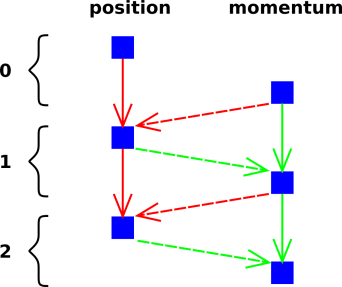
\includegraphics[width=0.8\textwidth]{images/integrator-symplectic-stagger.png}
                \caption{Symplectic integrator example: Velocity Verlet}
            \end{figure}
        \end{column}
    \end{columns}
    \footnotesize Source: \url{https://www.av8n.com/physics/symplectic-integrator.htm}
\end{frame}

\begin{frame}
    \frametitle{Methods - The Parareal Algorithm}

    \begin{columns}
        \begin{column}{0.4\textwidth}
            \begin{itemize}
                \item<1-> Can't traditionally parallelize initial value problems (IVP)
                \item<2-> Generate initial coarse solution
                \item<3-> Generate fine solution for each coarse IVP in parallel
                \item<4-> Correct coarse solution
                \item<5-> Loop
            \end{itemize}
        \end{column}
        \begin{column}{0.6\textwidth}
            \begin{figure}
                \centering
                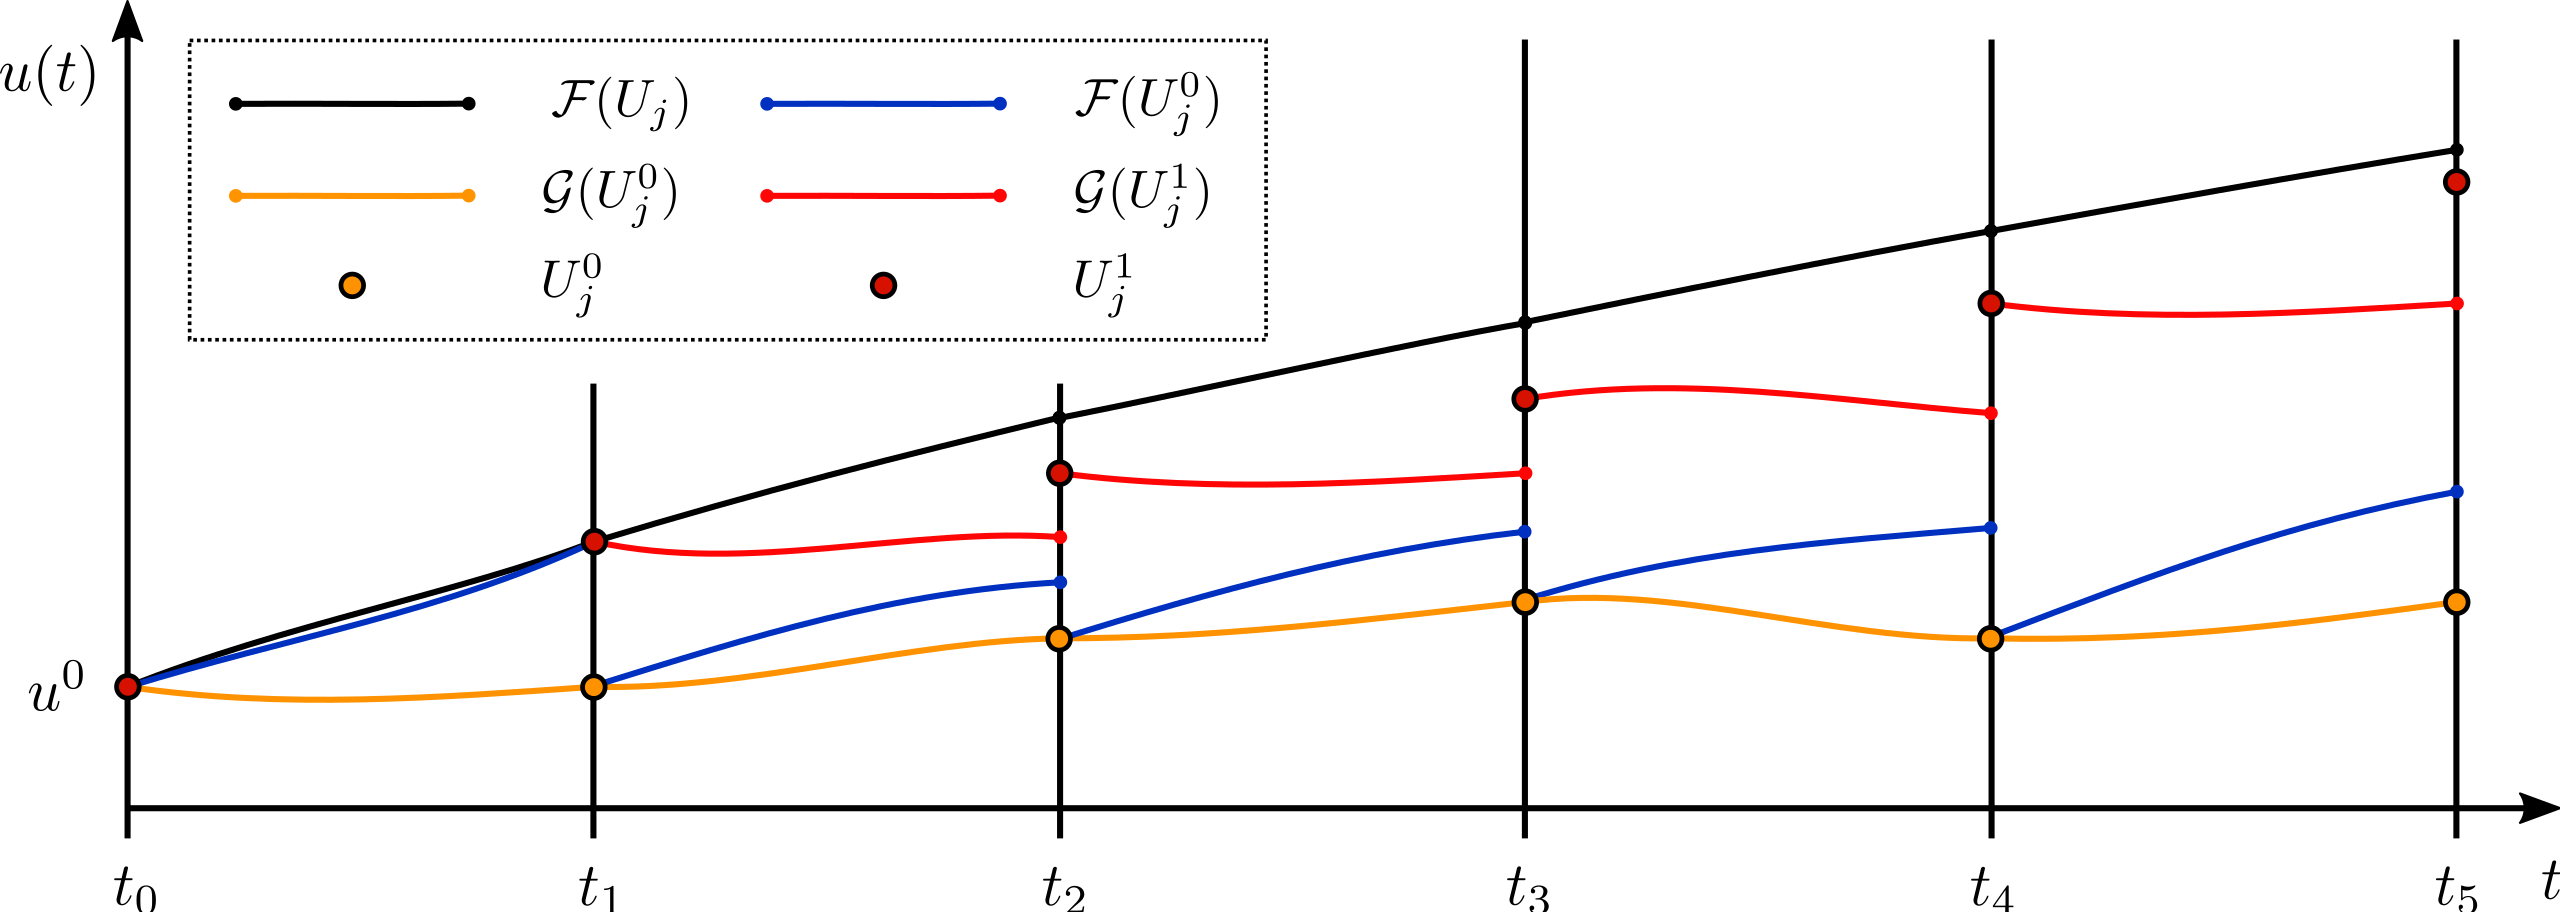
\includegraphics[width=\textwidth]{images/Parareal.png}
                \caption{Illustration of the first iteration in Parareal}
            \end{figure}
        \end{column}
    \end{columns}
    \vfill
    \footnotesize Source: \url{https://commons.wikimedia.org/wiki/File:Parareal.svg}
\end{frame}

\begin{frame}
    \frametitle{Methods - The Parareal Algorithm}

    \begin{figure}[h]
        \centering
        \movie[autostart,loop,showcontrols]{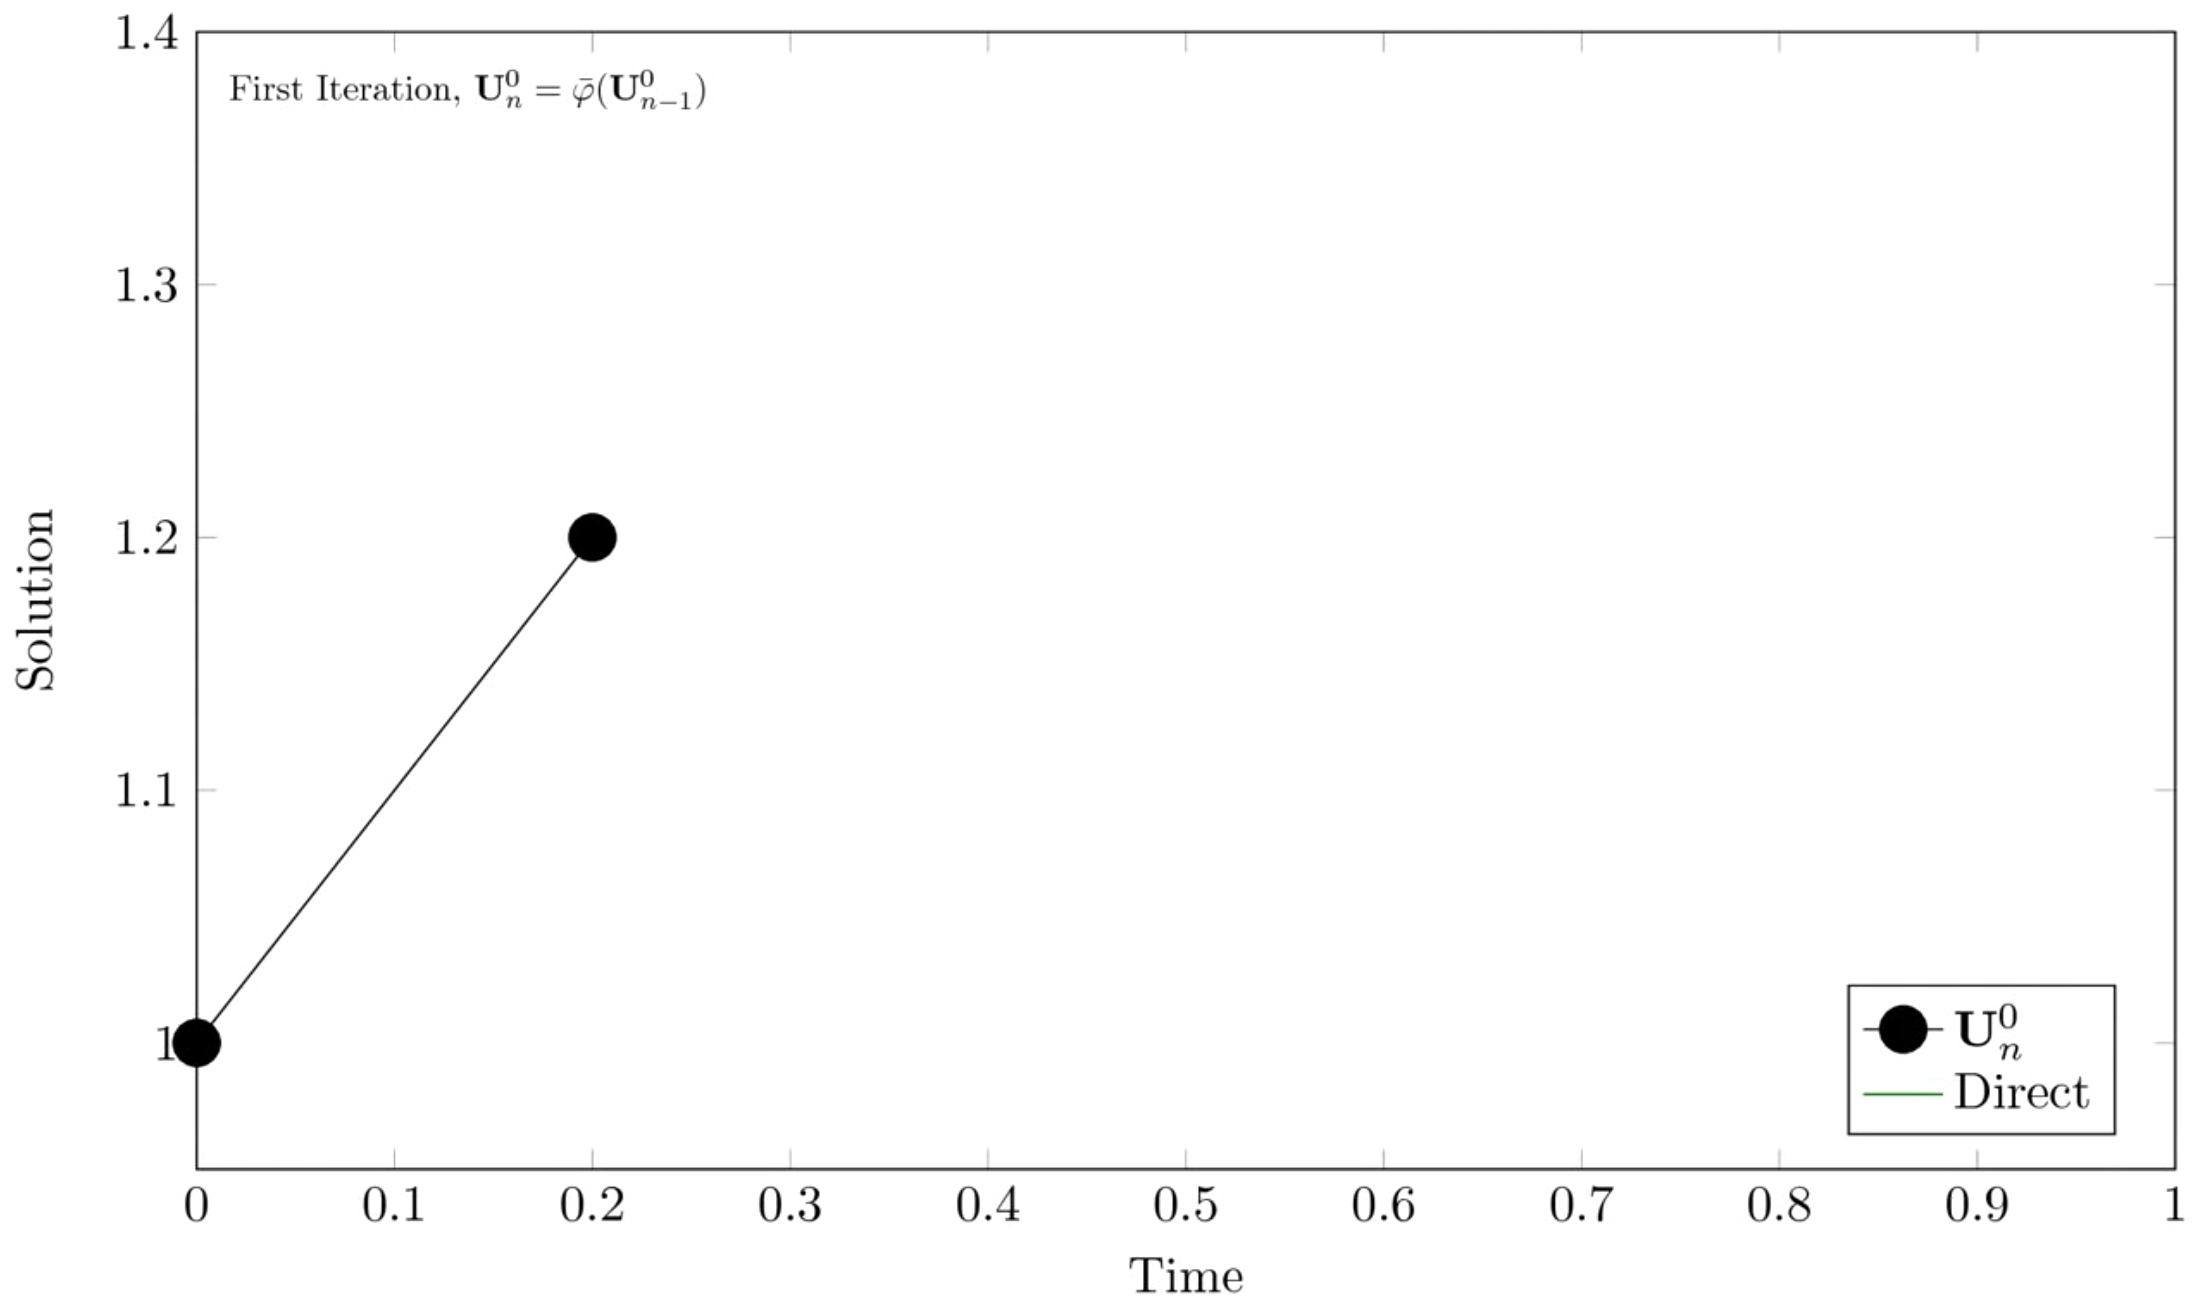
\includegraphics[height=0.7\textheight]{images/parareal_thumbnail.png}}{images/Parareal_Animation.ogx}
        \caption{The \textit{Parareal} approach to solving initial value problems in parallel.\\ Coarse: $\bar{\varphi}$, Fine: $\varphi$}
    \end{figure}
    \footnotesize Source: \url{https://en.wikipedia.org/wiki/File:Parareal_Animation.ogv}
\end{frame}

\begin{frame}
    \frametitle{Methods - High-Performance Computing}

    \begin{columns}
        \column{0.6\textwidth}
            \begin{itemize}
                \item <1->Equation for each $k < k_c$
                \item <2->Many equations to solve
                \item <3->Solve at the same time with multiple GPUs
                \item <4->Use CWU's ``Turing'' supercomputer
                \item <4->12 NVIDA P100 GPUs \\- Each 83\% performance of modern RTX 3060
                % \item 180 GBps GPU-GPU bandwidth
                % \item 80 GBps (NVLink) GPU-CPU bandwidth
            \end{itemize}
        \column{0.4\textwidth}
            \begin{figure}[h]
                \centering
                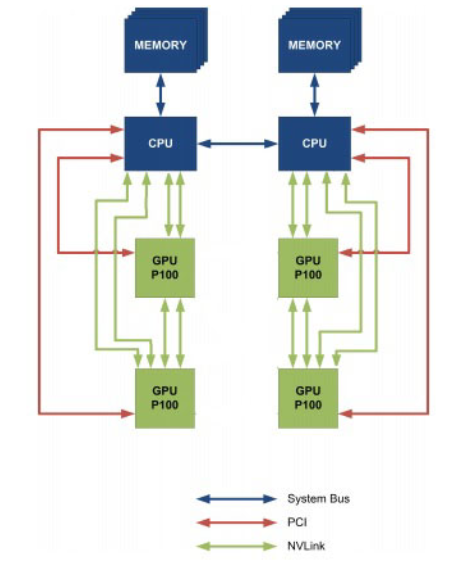
\includegraphics[height=0.65\textheight]{images/NVLink.png}
                \caption{CPU to GPU and GPU to GPU interconnect using NVLink}
            \end{figure}
    \end{columns}

\end{frame}
\section{Analytic Results}
\subsection{Final Time Distribution}
\begin{frame}
    \frametitle{Analytic Results - Simple Expansion}

    \begin{columns}
        \begin{column}{.5\textwidth}
            % \vspace{-0.5in}
            \begin{itemize}
                \item <1->Simple expansion: $a(t) = e^{-t/t_s}$
                \item <2->Use Mathematica for analytic results
                \item <3->Population distribution highly depends on length of expansion
                \item <4->Population is relatively high for low $k$
                \item <5->Population drops off quickly with $k$
            \end{itemize}
        \end{column}
        \begin{column}{.5\textwidth}
            \vspace{0.5in}
            \begin{figure}[h]
                \centering
                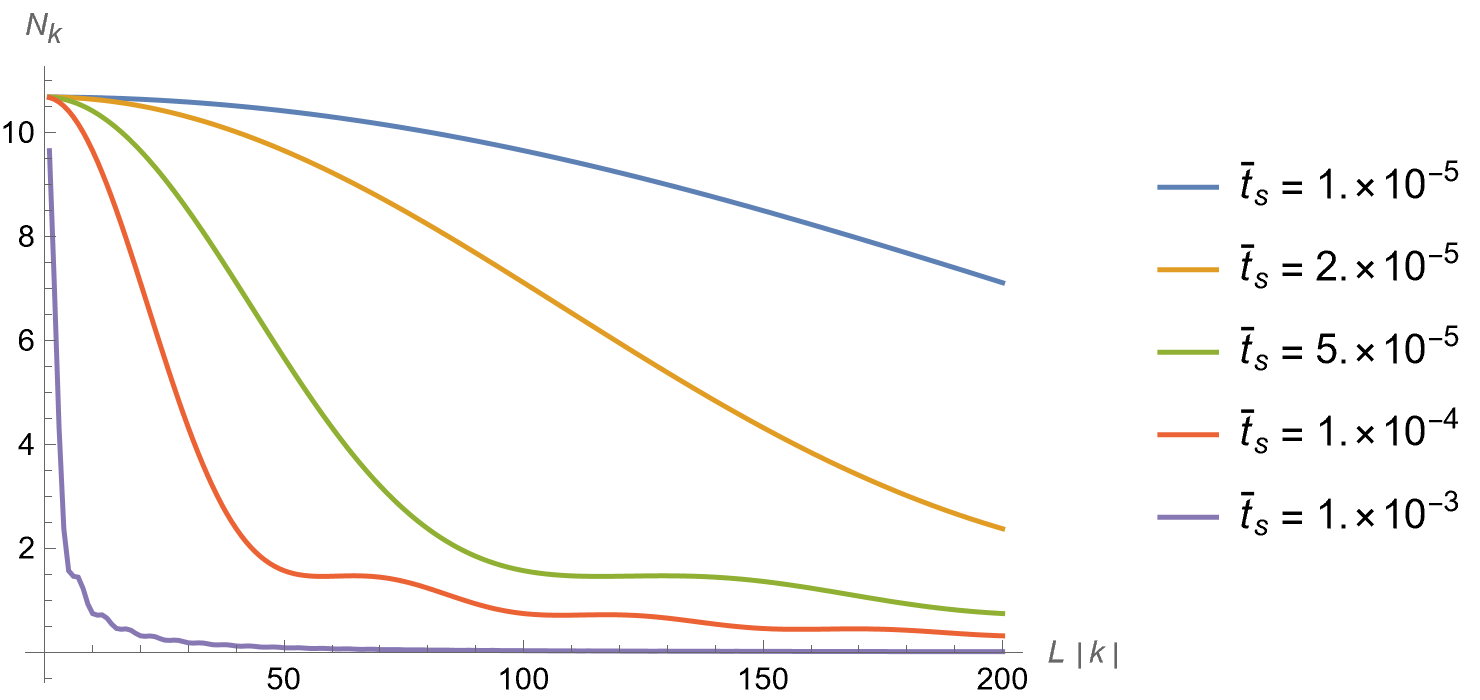
\includegraphics[width=\textwidth]{images/fig2.png}
                \caption{The momentum distribution when the universe stops expanding for multiple effective \\ rates of expansion}
                \label{fig:finalTime}
            \end{figure}
        \end{column}
    \end{columns}
\end{frame}

\begin{frame}
    \frametitle{Conclusion}
    \setstretch{1.25}
    \begin{itemize}
        \item <1->An inflating universe looks the same as an ultra-cold quantum gas with a decreasing speed of sound
        \item <2->Theory suggests inflation particles behave the same as ultra-cold quantum gases in the lab
        \item <3->There are many equations that need to be solved with special methods to conserve energy
        \item <4->Use high-performance techniques and hardware for reasonable execution time
        \item <5->Expect the distribution of momenta to depend on the length of the expansion
        \item <6->Expect the population to be high for low $k$ and drop off quickly
    \end{itemize}
\end{frame}

\begin{frame}
    \frametitle{Acknowledgements}

    \begin{itemize}
        \item Dr. Andy Piacsek (CWU, Physics)
        \item Dr. Szilard VAJDA (CWU, Computer Science)
        \item Dr. Micheal Braunstein (CWU, Physics)
        \item Dr. Brandon Peden (WWU, Physics \& Astronomy)
    \end{itemize}

\end{frame}

\begin{frame}{Thank you \& Code source}
    \begin{columns}[onlytextwidth]
        \begin{column}{.5\textwidth}
            Thank you for your attention.
            \vspace*{0.1\textheight} \\
            The code for this project is available at:
            \begin{itemize}
                \item GitHub (QR code): \url{github.com/nondairyneutrino/thesis}
                \item My website: \url{nathanwchapman.com}
            \end{itemize}
        \end{column}
        \begin{column}{.5\textwidth}
            \centering
            \qrcode[height=0.67\textheight]{https://github.com/nondairyneutrino/thesis}
        \end{column}
    \end{columns}
    \end{frame}

\subsection{All Time Distribution}
\begin{frame}
    \frametitle{Analytic Results - Simple Expansion}

    \begin{figure}[h]
        \centering
        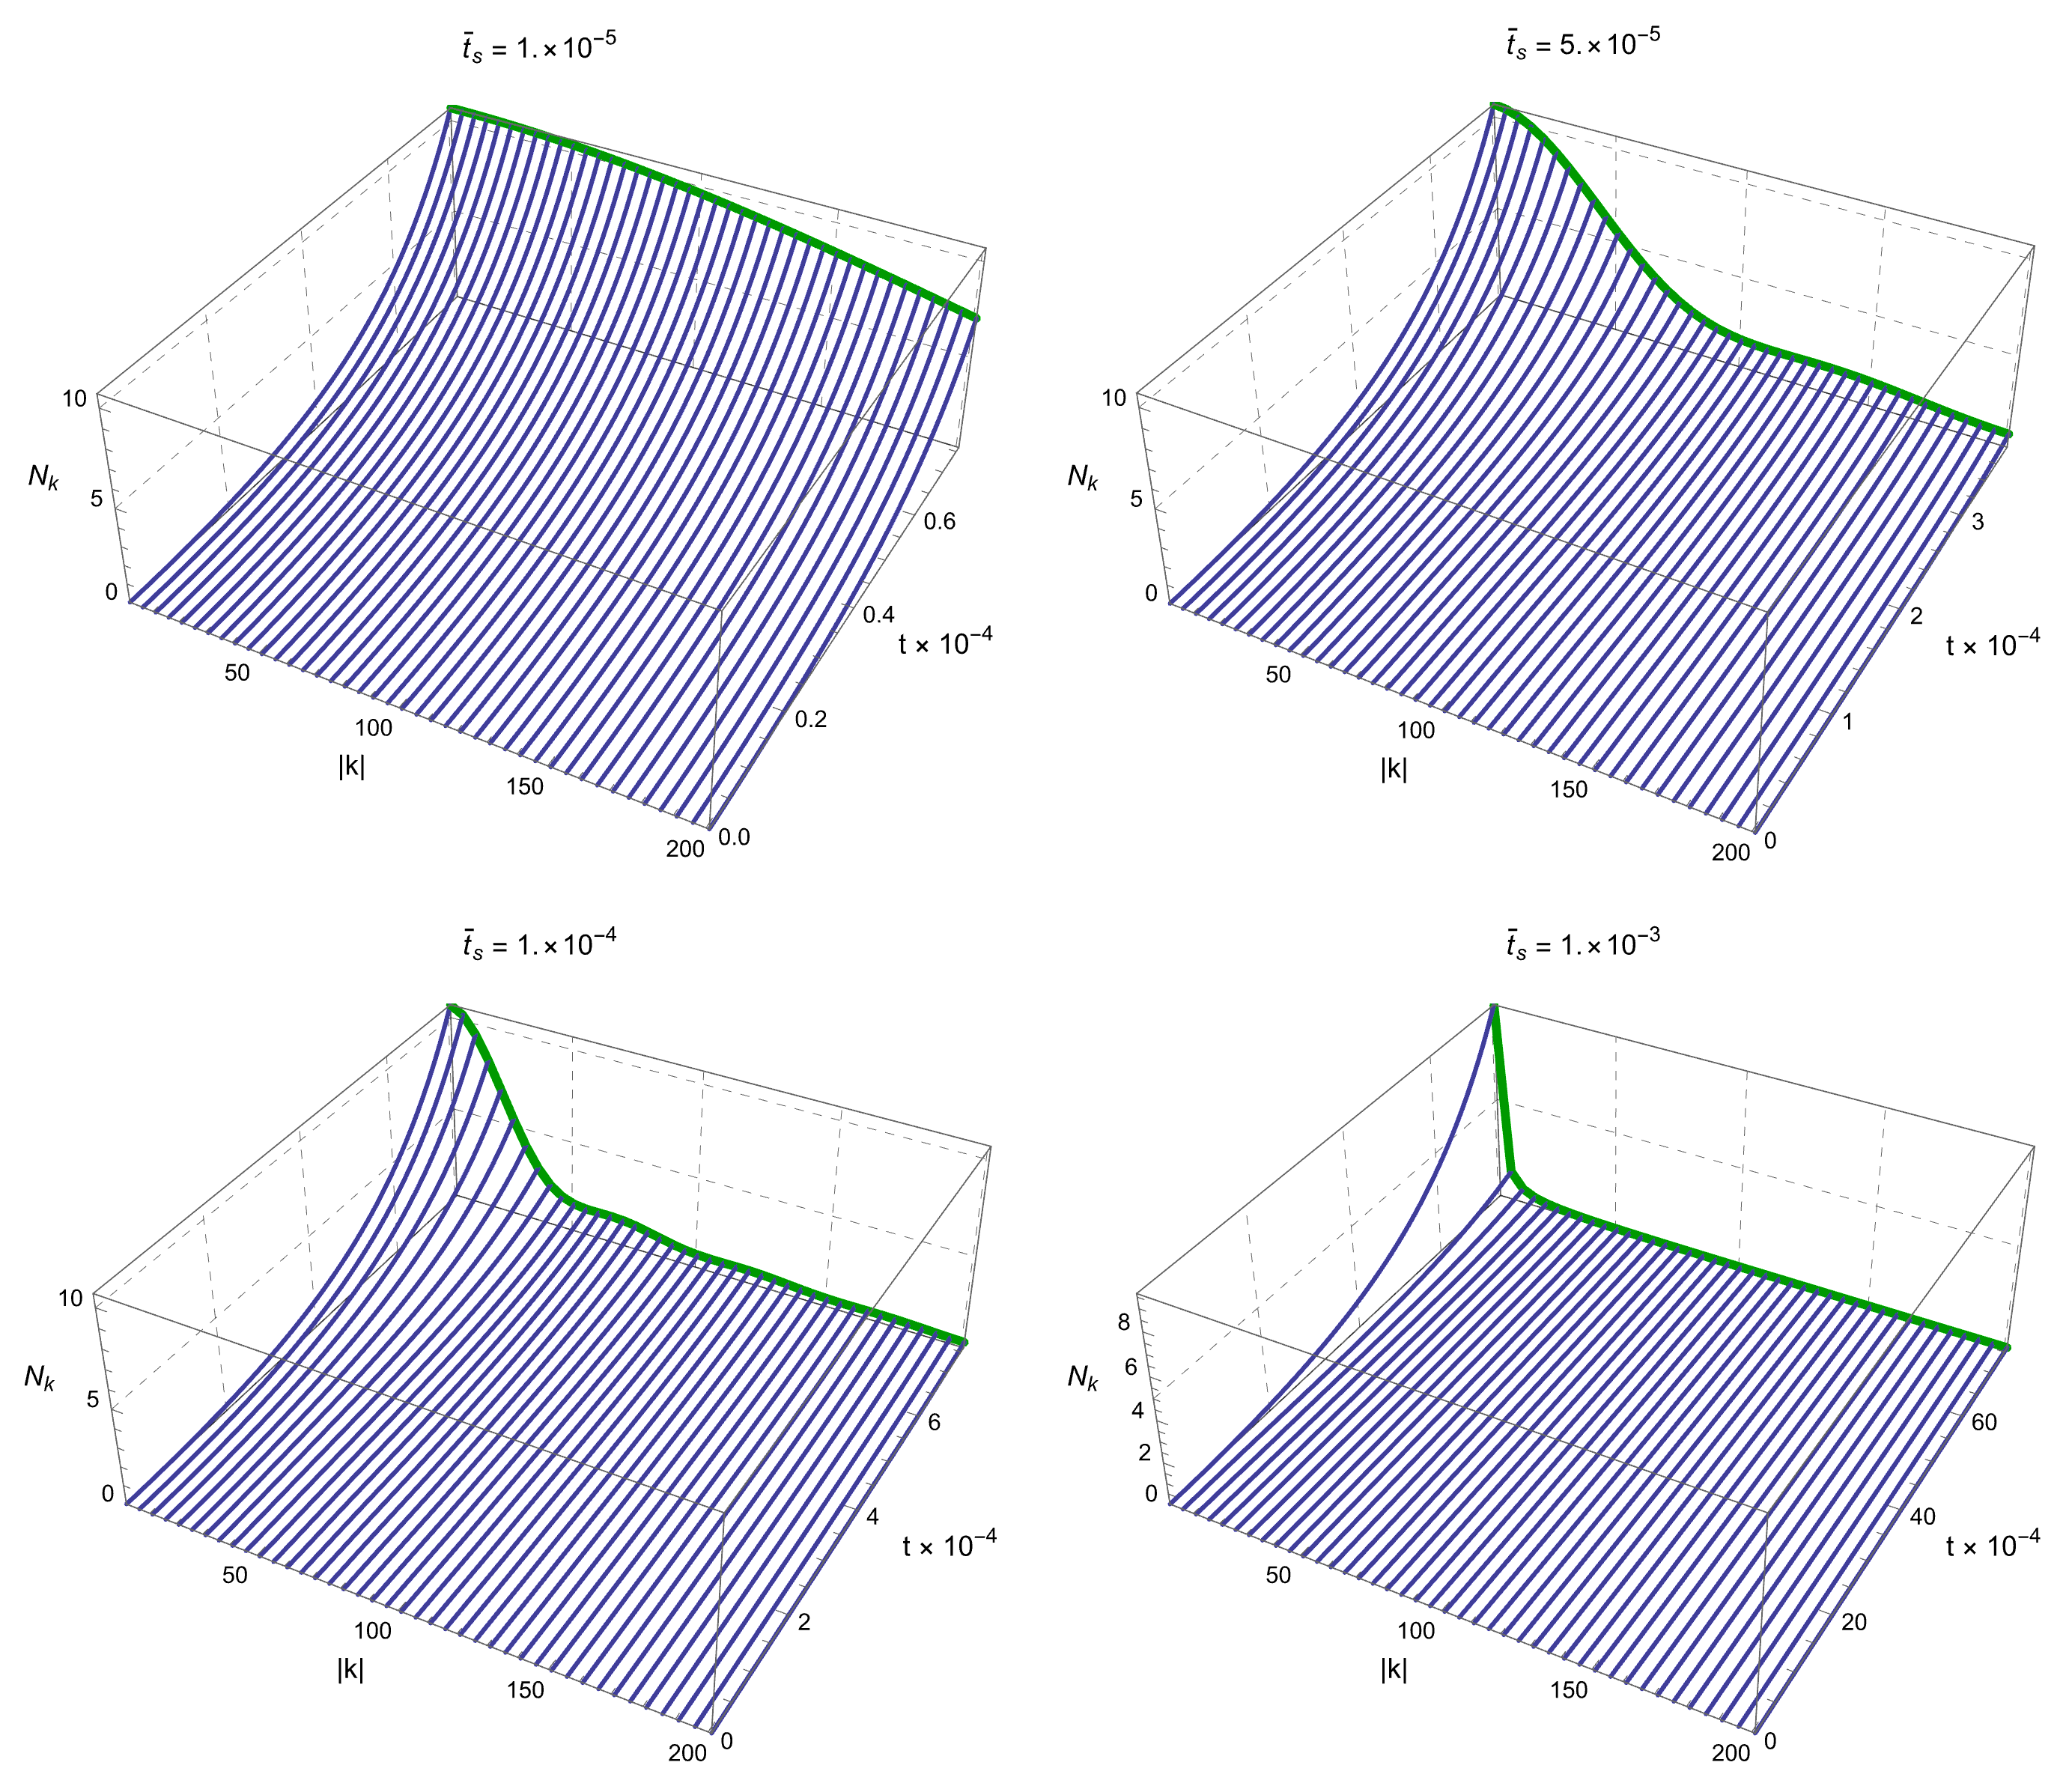
\includegraphics[height=0.74\textheight]{images/Analytic_Fig_4.png}
        \caption{Momentum distribution throughout the expansion}
        \label{fig:allTime}
    \end{figure}

\end{frame}

% \begin{frame}[allowframebreaks]
%     \frametitle{\bibname}
%     \nocite{*}
%     \printbibliography
% \end{frame}

\end{document}